% Chapter 3, Topic _Linear Algebra_ Jim Hefferon
%  http://joshua.smcvt.edu/linearalgebra
%  2001-Jun-12
\topic{Garis Kecocokan Terbaik}
\index{kuadrat terkecil|(}
\index{garis kecocokan terbaik|(}
\index{persamaan linear!sistem tak konsisten}
\textit{Topik ini memerlukan rumus-rumus dari subbagian Proyeksi Ortogonal ke
        Garis dan Proyeksi ke Subruang.}

Ilmuwan sering berhadapan dengan sistem yang tidak memiliki solusi, tetapi tetap
harus menemukan jawaban. Lebih tepatnya, mereka harus menemukan jawaban terbaik.
Sebagai contoh, berikut adalah hasil pelemparan sekeping uang logam, termasuk
beberapa hasil antara.
\begin{center} \small
  \begin{tabular}{r|ccc}
     \textit{banyak lemparan}  &30  &60  &90   \\
     \hline
     \textit{banyak sisi kepala}  &16  &34  &51
  \end{tabular}
\end{center}
Karena percobaan ini bersifat acak, kita mengharapkan proporsi sisi kepala
terhadap banyak lemparan berfluktuasi di sekitar nilai jangka panjang $50\%$.
Jadi, sistem bagi percobaan semacam itu mungkin tidak memiliki solusi, dan
itulah yang terjadi di sini.
\begin{equation*}
  \begin{linsys}{1}
    30m  &=  &16    \\
    60m  &=  &34    \\
    90m  &=  &51
  \end{linsys}
\end{equation*}
Artinya, vektor data yang kita kumpulkan tidak berada dalam subruang tempat
vektor itu semestinya berada secara ideal.
\begin{equation*}
  \colvec{16 \\ 34 \\ 51}\not\in
    \set{ m\colvec{30 \\ 60 \\ 90}  \suchthat m\in\Re}
\end{equation*}
Namun, kita tetap harus memperoleh sesuatu, sehingga kita mencari~$m$ yang
paling mendekati kecocokan. Proyeksi ortogonal vektor data ke subruang garis
memberikan taksiran terbaik, yaitu vektor dalam subruang yang paling dekat dengan
vektor data.
\begin{equation*}
  \frac{ \colvec[r]{16 \\ 34 \\ 51}\dotprod\colvec[r]{30 \\ 60 \\ 90} }{
           \colvec[r]{30 \\ 60 \\ 90}\dotprod\colvec[r]{30 \\ 60 \\ 90} }
     \cdot\colvec[r]{30 \\ 60 \\ 90}
  =\frac{7110}{12600}\cdot \colvec[r]{30 \\ 60 \\ 90}
\end{equation*}
Taksiran (\( m=7110/12600\approx 0.56 \)) sedikit lebih besar daripada
setengah, tetapi tidak jauh lebih besar, sehingga uang logam tersebut agaknya
cukup seimbang.

Garis dengan kemiringan \( m\approx 0.56 \) merupakan
\definend{garis kecocokan terbaik}\index{garis!kecocokan terbaik}%
\index{garis kecocokan terbaik} bagi data ini.
\begin{center}  \small
  \includegraphics{map/mp/ch3.42}
\end{center}
Meminimumkan jarak antara vektor yang diberikan dan vektor yang digunakan
sebagai ruas kanan meminimumkan jumlah kuadrat panjang vertikal ini. Karena itu, kita
mengatakan bahwa garis tersebut diperoleh melalui
\definend{pencocokan dengan kuadrat terkecil}.\index{kuadrat terkecil}
\begin{center}  \small
  \includegraphics{map/mp/ch3.43}
\end{center}
Diagram ini memperbesar skala vertikal dengan faktor sepuluh agar panjangnya
lebih mudah terlihat.

Dalam persamaan di atas, garis harus melalui \( (0,0) \) karena kita menganggap
kemiringannya sebagai proporsi sebenarnya antara sisi kepala dan banyak lemparan
uang logam tersebut. Kita juga dapat menangani kasus ketika garis tidak harus
melalui titik asal.

Berikut adalah perkembangan catatan waktu rekor dunia lari satu mil putra
\cite{Oakley}. Pada awal 1900-an banyak orang bertanya-tanya kapan, atau bahkan
apakah, rekor tersebut akan menembus batas empat menit.
Berikut adalah catatan waktu yang berlaku pada tanggal satu Januari setiap
dasawarsa sepanjang paruh pertama abad itu.
\begin{center} \small
  \begin{tabular}{r|ccccccccc}
    \textit{tahun} &$1870$ &$1880$ &$1890$  &$1900$
        &$1910$  &$1920$  &$1930$ &$1940$ &$1950$   \\
    \hline
    \textit{detik}  &$268.8$  &$264.5$  &$258.4$  &$255.6$
        &$255.6$  &$252.6$  &$250.4$ &$246.4$ &$241.4$
  \end{tabular}  
\end{center}
Kita dapat menggunakan data ini untuk membuat prediksi sekitar tahun 1950
tentang kapan catatan $240$ detik akan tercapai, lalu membandingkannya dengan
tanggal sebenarnya. Seperti data uang logam, bilangan-bilangan ini tidak
terletak tepat pada satu garis. Artinya, sistem berikut tidak memiliki solusi
eksak bagi kemiringan dan intersep.
\begin{equation*}
  \begin{linsys}{2}
    b &+  &1870m  &=  &268.8 \\ 
    b &+  &1880m  &=  &264.5 \\ 
      &   &       &\vdots     \\
    b &+  &1950m  &=  &241.4  
  \end{linsys}
\end{equation*}
Kita menemukan hampiran terbaik dengan menggunakan proyeksi ortogonal.

(\textit{Catatan tentang data.}
Pembatasan pada catatan waktu di awal setiap dasawarsa mengurangi beban
memasukkan data, menghaluskan data sampai taraf tertentu, dan memberikan hasil
yang hampir sama dengan memasukkan semua tanggal dan rekor.
Terdapat beberapa urutan catatan waktu dari badan standar yang saling bersaing,
tetapi data di sini berasal dari \cite{WikipediaMensMile}.
Plot dimulai pada 1870 karena pada suatu masa terdapat dua kelas rekor, yang
disebut `profesional' dan `amatir'. Setelah beberapa waktu kelas pertama tidak
lagi aktif, sehingga kita mengikuti kelas kedua.)

Tuliskan matriks koefisien sistem linear tersebut beserta vektor konstantanya,
yaitu catatan waktu rekor dunia.
\begin{equation*}
  A=
  \begin{mat}
    1  &1870  \\
    1  &1880  \\
    \vdots  &\vdots \\
    1  &1950  
  \end{mat}
  \qquad
  \vec{v}=\colvec{268.8 \\ 264.5 \\ \vdots \\ 241.4}
\end{equation*}
Hasil terakhir dalam subbagian Proyeksi ke Subruang memberikan rumus bagi
koefisien $b$ dan $m$ yang membuat kombinasi linear kolom-kolom $A$ sedekat
mungkin dengan $\vec{v}$.
Koefisien-koefisien itu merupakan entri vektor
$(\trans{A}A)^{-1}\trans{A}\cdot\vec{v}$.

\textit{Sage} dapat menjalankan perhitungannya bagi kita.
\begin{lstlisting}
sage: year = [1870, 1880, 1890, 1900, 1910, 1920, 1930, 1940, 1950]
sage: secs = [268.8, 264.5, 258.4, 255.6, 255.6, 252.6, 250.4, 246.4, 241.4]
sage: var('a, b, t')
(a, b, t)
sage: model(t) = a*t+b
sage: data = zip(year, secs)
sage: fit = find_fit(data, model, solution_dict=True)
sage: model.subs(fit)
t |--> -0.3048333333333295*t + 837.0872222222147
sage: g=points(data)+plot(model.subs(fit),(t,1860,1960),color='red',
....:                     figsize=3,fontsize=7,typeset='latex')
sage: g.save("four_minute_mile.pdf")
sage: g
\end{lstlisting}

\begin{center}  
  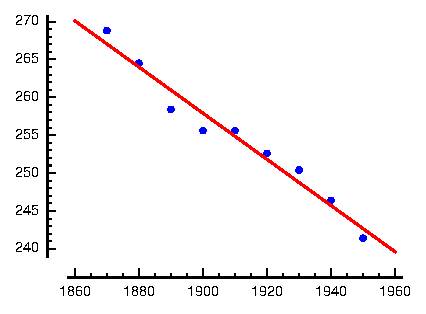
\includegraphics[width=0.5\textwidth]{map/pix/four_minute_mile.pdf}
\end{center}
Perkembangan tersebut membentuk garis yang sangat baik secara mengejutkan.
Dari kemiringan dan intersepnya kita memprediksi $1958.73$; tanggal sebenarnya
rekor Roger Bannister adalah 6 Mei 1954.

Contoh terakhir membandingkan gaji tim liga utama bisbol Amerika Serikat dengan
banyak kemenangan tim pada tahun 2002.
Pada tahun itu, Oakland Athletics menggunakan teknik matematis untuk
mengoptimalkan pemain yang diturunkan sesuai dana yang dapat dibelanjakan,
seperti diceritakan dalam film \textit{Moneyball}.
(Gaji dinyatakan dalam juta dolar dan banyak kemenangan dihitung dari 162
pertandingan.)

Untuk menjalankan perhitungan, sekali lagi kita menggunakan \textit{Sage}.
% http://ask.sagemath.org/question/768/fitting-a-curve-to-a-straight-line?answer=1271#1271
% by Joaquim Puig on 2011-Sep-27; gathered on 2013-Oct-23 JH
\begin{lstlisting}
sage: sal = [40, 40, 39, 42, 45, 42, 62, 34, 41, 57, 58, 63, 47, 75, 57, 78, 80, 50, 60, 93,
....:        77, 55, 95, 103, 79, 76, 108, 126, 95, 106]
sage: wins = [103, 94, 83, 79, 78, 72, 99, 55, 66, 81, 80, 84, 62, 97, 73, 95, 93, 56, 67,
....:        101, 78, 55, 92, 98, 74, 67, 93, 103, 75, 72]
sage: var('a, b, t')
(a, b, t)
sage: model(t) = a*t+b
sage: data = zip(sal,wins)
sage: fit = find_fit(data, model, solution_dict=True)
sage: model.subs(fit)
t |--> 0.2634981251436269*t + 63.06477642781477
sage: p = points(data,size=25)+plot(model.subs(fit),(t,30,130),color='red',typeset='latex')
sage: p.save('moneyball.pdf')
\end{lstlisting}

Grafiknya ditampilkan di bawah.
Tim di kiri atas, yang membayar sedikit untuk memperoleh banyak kemenangan,
adalah Oakland A's.

\begin{center}  \small
  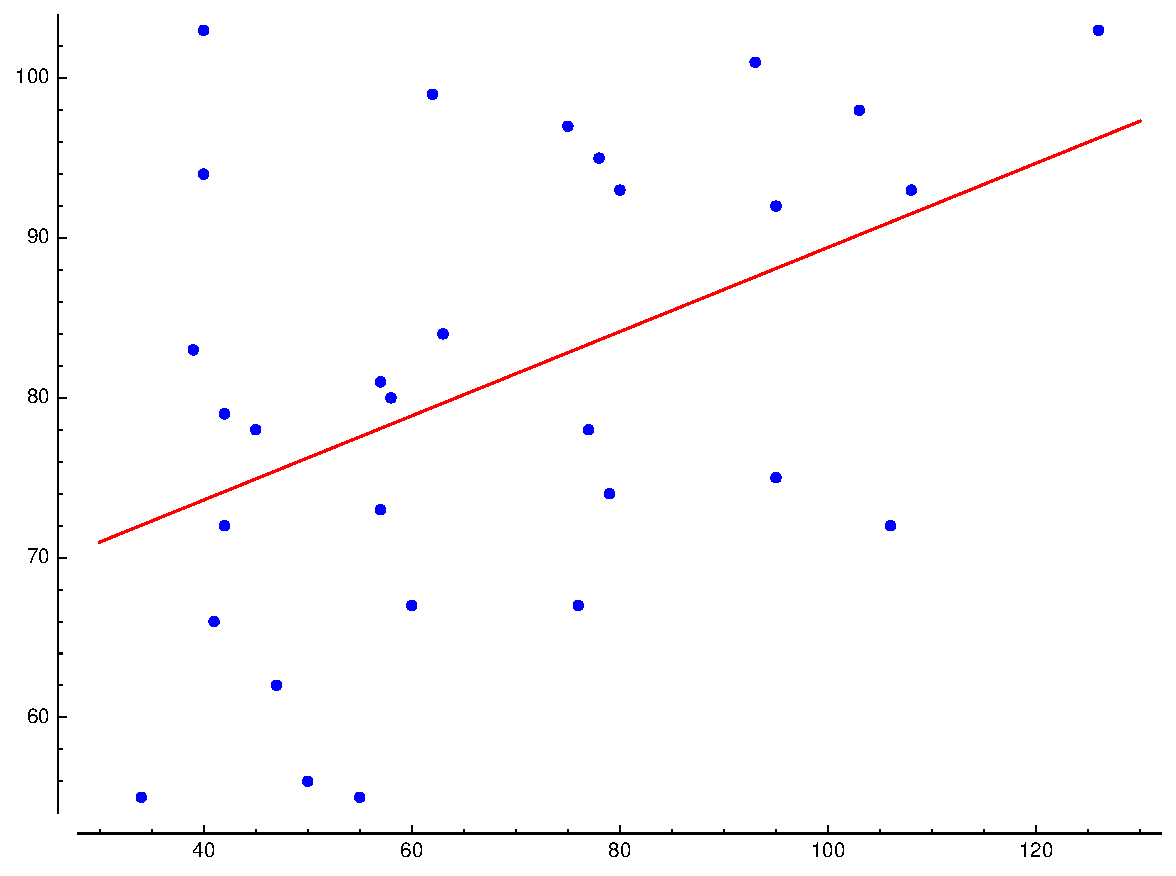
\includegraphics[width=0.5\textwidth]{map/pix/moneyball.pdf}
\end{center}

Menilai garis ini hanya dengan mata rentan terhadap kesalahan.
Karena itu, persamaan-persamaan tersebut memberi kita kepastian tentang makna
`terbaik' dalam kecocokan terbaik.
Selain itu, persamaan model secara kasar menyatakan bahwa dengan membelanjakan
satu juta dolar tambahan, pemilik tim dapat berharap membeli $1/4$ kemenangan
(dan syukurlah, harapan itu tidak terlalu pasti).


% For example, the different denominations of US\ money have different average 
% times in circulation.\cite{FedReserve}
% (The $\$2$~bill is a special case because 
% Americans mistakenly believe that 
% it is collectible and do not circulate these bills.)
% \begin{lstlisting}
% sage: x = [1, 5, 10, 20, 50, 100]
% sage: y = [5.9, 4.9, 4.2, 7.7, 3.7, 15.0]
% sage: var('a, b, t') 
% (a, b, t)
% sage: model(t) = a*t+b
% sage: data = zip(x,y)
% sage: fit = find_fit(data, model, solution_dict=True)
% sage: model.subs(fit)                                
% t |--> 0.08650137692301652*t + 4.2184573359365265
% sage: plot(model.subs(fit),(t,0,100))+points(data,size=20,color='red')
% \end{lstlisting}  
% How long should a $\$25$~bill last?

% \begin{center}  \small
%   \includegraphics[width=0.5\textwidth]{map/pix/denom.png}
% \end{center}


% \begin{center}  \small
%   \begin{tabular}{r|cccccc}
%      \textit{denomination}          
%         &$1$   &$5$    &$10$     &$20$     &$50$     &$100$ \\
%       \hline
%      \textit{average life (mos)}  
%         &$22.0$ &$15.9$  &$18.3$   &$24.3$   &$55.4$   &$88.8$  \\
%   \end{tabular}
% \end{center}
% The data plot below looks roughly linear.
% It isn't a perfect line, i.e.,
% the linear system with equations $b+1m=1.5$, \ldots, $b+100m=20$ has no 
% solution, but we can again use orthogonal projection 
% to find a best approximation.
% Consider the matrix of coefficients of that linear system and also its
% vector of constants, the experimentally-determined values.
% \begin{equation*}
%   A=
%   \begin{mat}[r]
%     1  &1  \\
%     1  &5  \\
%     1  &10  \\
%     1  &20  \\
%     1  &50  \\
%     1  &100  
%   \end{mat}
%   \qquad
%   \vec{v}=\colvec[r]{22.0 \\ 15.9 \\ 18.3 \\ 24.3 \\ 55.4 \\ 88.8}
% \end{equation*}
% The ending result in the subsection on Projection into a Subspace says
% that coefficients $b$ and $m$ so that the linear combination
% of the columns of $A$ is as close as possible to the vector $\vec{v}$ 
% are the entries of $(\trans{A}A)^{-1}\trans{A}\cdot\vec{v}$.
% Some calculation
% gives an intercept of $b=14.16$ and a slope
% of $m= 0.75$.
% \begin{center}  \small
%   \includegraphics{map/mp/ch3.44}
% \end{center}
% Plugging $x=25$ into the equation of the line shows that such a 
% bill should last about two and three-quarters years.


%
%
%We want to project when a 3:40~mile %\hrsmins{3}{40} 
%will be run.
%\begin{center}
%  \begin{tabular}{r|ccccccc}
%    \textit{year} &1870  &1880  &1890  &1900  &1910  &1920  &1930   \\
%    \hline
%    \textit{secs}  &$268.8$  &$264.5$  &$258.4$  &$255.6$  
%        &$255.6$  &$252.6$  &$250.4$
%  \end{tabular}        \\[2ex]
%  \begin{tabular}{|ccccccc}
%      1940  &1950  &1960  &1970  &1980  &1990 &2000                  \\
%      \hline
%      $246.4$  &$241.4$  &$234.5$  &$231.1$  &$229.0$  &$226.3$ &$223.1$
%  \end{tabular}
%\end{center}
%We can see below that the data is surprisingly linear.
%With this input
%\begin{equation*}
%  A= 
%  \begin{mat}
%    1 & 1860 \\
%    1 & 1870 \\
%%    1 & 1880 \\
%%    1 & 1890 \\ 
%%    1 & 1900 \\ 
%%    1 & 1910 \\
%%    1 & 1920 \\
%%    1 & 1930 \\
%%    1 & 1940 \\
%%    1 & 1950 \\
%%    1 & 1960 \\
%%    1 & 1970 \\
%%    1 & 1980 \\
%    \vdots &\vdots  \\
%    1 &1990  \\
%    1 &2000
%  \end{mat}
%  \qquad
%  \vec{v} = \colvec{280.0 \\
%                    268.8 \\
%%                    264.5 \\
%%                    258.4 \\
%%                    255.6 \\
%%                    255.6 \\
%%                    252.6 \\
%%                    250.4 \\
%%                    246.4 \\
%%                    241.4 \\
%%                    234.5 \\
%%                    231.1 \\
%%                    229.0 \\
%                    \vdots \\
%                    226.3 \\
%                    223.1}
%\end{equation*}
%%MAPLE gives $b=970.68$ and $m=-0.37$  (rounded to two places).
%the Python program at this Topic's end gives 
%%$\text{slope}= -0.351428571429$
%%and $\text{intercept}= 925.534065934$ 
%$\text{slope}= -0.35$
%and $\text{intercept}= 925.53$ 
%(rounded to two places; the original data 
%is good to only about a quarter of a second 
%since much of it was hand-timed).
%\begin{center}  \small
%  \includegraphics{map/mp/ch3.45}
%\end{center}
%When will a \( 220 \) second mile be run?
%Solving the equation of the line of best fit 
%gives an estimate of the year \( 2008 \).
%
%This example is amusing, but serves as a caution \Dash obviously the 
%linearity of the data will break down someday (as indeed it does 
%prior to 1860).



\begin{exercises}
  \item[]\emph{Perhitungan di sini paling baik dijalankan dengan komputer.
      Beberapa soal memerlukan data dari Internet.}
%   \begin{Filesave}{bookans}  % write the records to the answer file.
%     \textit{Data on the progression of the world's records 
%        (taken from the \textit{Runner's World} web site)       
%        is below.}
%     \begin{figure}
%       \rotatebox[origin=lb]{90}{\hbox{\scriptsize
%         \begin{tabular}[t]{|l|ll|}
% %        \hline
% %          \multicolumn{3}{|c|}{\textit{Amateurs}}    \\
%         \hline
%           \multicolumn{3}{|c|}{\textit{Progression of Men's Mile Record}}  \\
%         \hline
%         \textit{time}  &\textit{name}  &\textit{date}  \\
%          \hline  
%            $\text{4:52}.0$      &Cadet Marshall (GBR)       &02Sep52 \\
%            $\text{4:45}.0$      &Thomas Finch (GBR)         &03Nov58 \\
%            %$\text{4:45}.0$      &St.~Vincent Hammick (GBR)  &15Nov58 \\
%            $\text{4:40}.0$      &Gerald Surman (GBR)        &24Nov59 \\
%            $\text{4:33}.0$      &George Farran (IRL)        &23May62 \\
%            $\text{4:29}\;3/5$   &Walter Chinnery (GBR)      &10Mar68 \\
%            $\text{4:28}\;4/5$   &William Gibbs (GBR)        &03Apr68 \\ 
%            $\text{4:28}\;3/5$   &Charles Gunton (GBR)       &31Mar73 \\
%            $\text{4:26}.0$      &Walter Slade (GBR)         &30May74 \\
%            $\text{4:24}\;1/2$   &Walter Slade (GBR)         &19Jun75 \\
%            $\text{4:23}\;1/5$   &Walter George (GBR)        &16Aug80 \\
%            $\text{4:19}\;2/5$   &Walter George (GBR)        &03Jun82 \\
%            $\text{4:18}\;2/5$   &Walter George (GBR)        &21Jun84 \\
%            $\text{4:17}\;4/5$   &Thomas Conneff (USA)       &26Aug93 \\
%            $\text{4:17}.0$      &Fred Bacon (GBR)           &06Jul95 \\
%            $\text{4:15}\;3/5$   &Thomas Conneff (USA)       &28Aug95 \\
%            $\text{4:15}\;2/5$   &John Paul Jones (USA)      &27May11 \\
%            $\text{4:14}.4$      &John Paul Jones (USA)      &31May13 \\
%            $\text{4:12}.6$      &Norman Taber (USA)         &16Jul15 \\
%            $\text{4:10}.4$      &Paavo Nurmi (FIN)          &23Aug23 \\
%            $\text{4:09}\;1/5$   &Jules Ladoumegue (FRA)     &04Oct31 \\
%            $\text{4:07}.6$      &Jack Lovelock (NZL)        &15Jul33 \\
%            $\text{4:06}.8$      &Glenn Cunningham (USA)     &16Jun34 \\
%            $\text{4:06}.4$      &Sydney Wooderson (GBR)     &28Aug37 \\
%            $\text{4:06}.2$      &Gunder Hagg (SWE)          &01Jul42 \\
%            %$\text{4:06}.2$      &Arne Andersson (SWE)       &10Jul42 \\
%            $\text{4:04}.6$      &Gunder Hagg (SWE)          &04Sep42 \\
%            $\text{4:02}.6$      &Arne Andersson (SWE)       &01Jul43 \\
%            $\text{4:01}.6$      &Arne Andersson (SWE)       &18Jul44 \\
%            $\text{4:01}.4$      &Gunder Hagg (SWE)          &17Jul45 \\
%            $\text{3:59}.4$      &Roger Bannister (GBR)      &06May54 \\
%            $\text{3:58}.0$      &John Landy (AUS)           &21Jun54 \\
%            $\text{3:57}.2$      &Derek Ibbotson (GBR)       &19Jul57 \\
%            $\text{3:54}.5$      &Herb Elliott (AUS)         &06Aug58 \\
%            $\text{3:54}.4$      &Peter Snell (NZL)          &27Jan62 \\ 
%            $\text{3:54}.1$      &Peter Snell (NZL)          &17Nov64 \\
%            $\text{3:53}.6$      &Michel Jazy (FRA)          &09Jun65 \\
%            $\text{3:51}.3$      &Jim Ryun (USA)             &17Jul66 \\
%            $\text{3:51}.1$      &Jim Ryun (USA)             &23Jun67 \\
%            $\text{3:51}.0$      &Filbert Bayi (TAN)         &17May75 \\
%            $\text{3:49}.4$      &John Walker (NZL)          &12Aug75 \\
%            $\text{3:49}.0$      &Sebastian Coe (GBR)        &17Jul79 \\
%            $\text{3:48}.8$      &Steve Ovett (GBR)          &01Jul80 \\
%            $\text{3:48}.53$     &Sebastian Coe (GBR)        &19Aug81 \\
%            $\text{3:48}.40$     &Steve Ovett (GBR)          &26Aug81 \\
%            $\text{3:47}.33$     &Sebastian Coe (GBR)        &28Aug81 \\
%            $\text{3:46}.32$     &Steve Cram (GBR)           &27Jul85 \\
%            $\text{3:44}.39$     &Noureddine Morceli (ALG)   &05Sep93 \\
% 	   $\text{3:43}.13$     &Hicham el Guerrouj (MOR)   &07Jul99 \\
%       \hline
%       \end{tabular}
%       \   %
%         \begin{tabular}[t]{|l|ll|}
%         \hline
%           \multicolumn{3}{|c|}{\textit{Progression of Men's $1500$~Meter Record}}  \\
%         \hline
%         \textit{time}  &\textit{name}  &\textit{date}  \\
%          \hline  
%          $\text{4:09}.0$   &John Bray (USA)        &30May00  \\
%          $\text{4:06}.2$   &Charles Bennett (GBR)  &15Jul00  \\
%          $\text{4:05}.4$   &James Lightbody (USA)  &03Sep04  \\
%          $\text{3:59}.8$   &Harold Wilson (GBR)    &30May08  \\
%          $\text{3:59}.2$   &Abel Kiviat (USA)      &26May12  \\
%          $\text{3:56}.8$   &Abel Kiviat (USA)      &02Jun12  \\
%          $\text{3:55}.8$   &Abel Kiviat (USA)      &08Jun12  \\
%          $\text{3:55}.0$   &Norman Taber (USA)     &16Jul15  \\
%          $\text{3:54}.7$   &John Zander (SWE)      &05Aug17  \\
%          $\text{3:53}.0$   &Paavo Nurmi (FIN)      &23Aug23  \\
%          $\text{3:52}.6$   &Paavo Nurmi (FIN)      &19Jun24  \\
%          $\text{3:51}.0$   &Otto Peltzer (GER)     &11Sep26  \\
%          $\text{3:49}.2$   &Jules Ladoumegue (FRA) &05Oct30  \\
%          %$\text{3:49}.2$   &Luigi Beccali (ITA)    &09Sep33  \\
%          $\text{3:49}.0$   &Luigi Beccali (ITA)    &17Sep33  \\
%          $\text{3:48}.8$   &William Bonthron (USA) &30Jun34  \\
%          $\text{3:47}.8$   &Jack Lovelock (NZL)    &06Aug36  \\
%          $\text{3:47}.6$   &Gunder Hagg (SWE)      &10Aug41  \\
%          $\text{3:45}.8$   &Gunder Hagg (SWE)      &17Jul42  \\
%          $\text{3:45}.0$   &Arne Andersson (SWE)   &17Aug43  \\
%          $\text{3:43}.0$   &Gunder Hagg (SWE)      &07Jul44  \\
%          %$\text{3:43}.0$   &Lennart Strand (SWE)   &15Jul47  \\
%          %$\text{3:43}.0$   &Werner Lueg (FRG)      &29Jun52  \\
%          %$\text{3:43}.0$   &Roger Bannister (GBR)  &06May54  \\
%          $\text{3:42}.8$   &Wes Santee (USA)       &04Jun54  \\
%          $\text{3:41}.8$   &John Landy (AUS)       &21Jun54  \\
%          $\text{3:40}.8$   &Sandor Iharos (HUN)    &28Jul55  \\
%          %$\text{3:40}.8$   &Laszlo Tabori (HUN)    &06Sep55  \\
%          %$\text{3:40}.8$   &Gunnar Nielsen (DEN)   &06Sep55  \\
%          $\text{3:40}.6$   &Istvan Rozsavolgyi (HUN) &03Aug56 \\
%          $\text{3:40}.2$   &Olavi Salsola (FIN)    &11Jul57  \\
%          %$\text{3:40}.2$   &Olavi Salonen (FIN)    &11Jul57  \\
%          $\text{3:38}.1$   &Stanislav Jungwirth (CZE) &12Jul57  \\
%          $\text{3:36}.0$   &Herb Elliott (AUS)     &28Aug58  \\
%          $\text{3:35}.6$   &Herb Elliott (AUS)     &06Sep60  \\
%          $\text{3:33}.1$   &Jim Ryun (USA)         &08Jul67  \\
%          $\text{3:32}.2$   &Filbert Bayi (TAN)     &02Feb74  \\
%          $\text{3:32}.1$   &Sebastian Coe (GBR)    &15Aug79  \\
%          %$\text{3:32}.1$   &Steve Ovett (GBR)      &15Jul80  \\  
%          $\text{3:31}.36$  &Steve Ovett (GBR)      &27Aug80  \\
%          $\text{3:31}.24$  &Sydney Maree (usa)     &28Aug83  \\
%          $\text{3:30}.77$  &Steve Ovett (GBR)      &04Sep83  \\
%          $\text{3:29}.67$  &Steve Cram (GBR)       &16Jul85  \\
%          $\text{3:29}.46$  &Said Aouita (MOR)      &23Aug85  \\ 
%          $\text{3:28}.86$  &Noureddine Morceli (ALG)  &06Sep92  \\
%          $\text{3:27}.37$  &Noureddine Morceli (ALG)  &12Jul95  \\
%          $\text{3:26}.00$  &Hicham el Guerrouj (MOR)  &14Jul98  \\
%      \hline
%      \end{tabular}
%       \   %
%         \begin{tabular}[t]{|l|ll|}
%         \hline
%           \multicolumn{3}{|c|}{\textit{Progression of Women's Mile Record}}  \\
%         \hline
%         \textit{time}  &\textit{name}  &\textit{date}  \\
%          \hline  
%            $\text{6:13}.2$    &Elizabeth Atkinson (GBR)    &24Jun21 \\
%            $\text{5:27}.5$    &Ruth Christmas (GBR)        &20Aug32 \\
%            $\text{5:24}.0$    &Gladys Lunn (GBR)           &01Jun36 \\
%            $\text{5:23}.0$    &Gladys Lunn (GBR)           &18Jul36 \\
%            $\text{5:20}.8$    &Gladys Lunn (GBR)           &08May37 \\
%            $\text{5:17}.0$    &Gladys Lunn (GBR)           &07Aug37 \\
%            $\text{5:15}.3$    &Evelyne Forster (GBR)       &22Jul39 \\
%            $\text{5:11}.0$    &Anne Oliver (GBR)           &14Jun52 \\
%            $\text{5:09}.8$    &Enid Harding (GBR)          &04Jul53 \\
%            $\text{5:08}.0$    &Anne Oliver (GBR)           &12Sep53 \\
%            $\text{5:02}.6$    &Diane Leather (GBR)         &30Sep53 \\
%            $\text{5:00}.3$    &Edith Treybal (ROM)         &01Nov53 \\
%            $\text{5:00}.2$    &Diane Leather (GBR)         &26May54 \\
%            $\text{4:59}.6$    &Diane Leather (GBR)         &29May54 \\
%            $\text{4:50}.8$    &Diane Leather (GBR)         &24May55 \\
%            $\text{4:45}.0$    &Diane Leather (GBR)         &21Sep55 \\
%            $\text{4:41}.4$    &Marise Chamberlain (NZL)    &08Dec62 \\
%            $\text{4:39}.2$    &Anne Smith (GBR)            &13May67 \\
%            $\text{4:37}.0$    &Anne Smith (GBR)            &03Jun67 \\
%            $\text{4:36}.8$    &Maria Gommers (HOL)         &14Jun69 \\
%            $\text{4:35}.3$    &Ellen Tittel (FRG)          &20Aug71 \\
%            $\text{4:34}.9$    &Glenda Reiser (CAN)         &07Jul73 \\
%            $\text{4:29}.5$    &Paola Pigni-Cacchi (ITA)    &08Aug73 \\
%            $\text{4:23}.8$    &Natalia Marasescu (ROM)     &21May77 \\
%            $\text{4:22}.1$    &Natalia Marasescu (ROM)     &27Jan79 \\
%            $\text{4:21}.7$    &Mary Decker (USA)           &26Jan80 \\
%            $\text{4:20}.89$   &Lyudmila Veselkova (SOV)    &12Sep81 \\
%            $\text{4:18}.08$   &Mary Decker-Tabb (USA)      &09Jul82 \\
%            $\text{4:17}.44$   &Maricica Puica (ROM)        &16Sep82 \\
%            $\text{4:15}.8$    &Natalya Artyomova (SOV)     &05Aug84 \\
%            $\text{4:16}.71$   &Mary Decker-Slaney (USA)    &21Aug85 \\
%            $\text{4:15}.61$   &Paula Ivan (ROM)            &10Jul89 \\
%            $\text{4:12}.56$   &Svetlana Masterkova (RUS)   &14Aug96 \\
%        \hline
%        \end{tabular}
%       }}  %end the rotatebox
%     \end{figure}
%   \end{Filesave}  
  \item
    Gunakan kuadrat terkecil untuk menilai apakah uang logam dalam percobaan ini
    seimbang.
    \begin{center}
      \begin{tabular}{r|ccccc}
         \textit{lemparan}  &8  &16  &24  &32  &40 \\
         \hline
         \textit{sisi kepala}  &4  &9   &13  &17  &20
      \end{tabular}
    \end{center}
    \begin{answer}
      Seperti pada contoh pertama di atas, kita berusaha menemukan $m$ terbaik
      untuk ``menyelesaikan'' sistem berikut.
      \begin{equation*}
        \begin{linsys}{5}
          8m  &=  &4  \\
          16m &=  &9  \\
          24m &=  &13 \\
          32m &=  &17 \\
          40m &=  &20
        \end{linsys}
      \end{equation*}
      Proyeksi ke subruang linear memberikan
      \begin{equation*}
        \frac{\colvec[r]{4 \\ 9 \\ 13 \\ 17 \\20}
          \dotprod
          \colvec[r]{8  \\ 16 \\ 24 \\ 32 \\ 40}}{%
          \colvec[r]{8  \\ 16 \\ 24 \\ 32 \\ 40}
          \dotprod
          \colvec[r]{8  \\ 16 \\ 24 \\ 32 \\ 40}}
        \cdot
        \colvec[r]{8  \\ 16 \\ 24 \\ 32 \\ 40}
        =
        \frac{1832}{3520}
        \cdot
        \colvec[r]{8  \\ 16 \\ 24 \\ 32 \\ 40}
      \end{equation*}
      sehingga kemiringan garis kecocokan terbaik kira-kira
      $1832/3520=0.52045$.
      Nilai ini dekat dengan $0.5$, sehingga data tersebut konsisten dengan uang
      logam yang cukup seimbang.
      \begin{center}  \small
        \includegraphics{map/mp/ch3.85}
      \end{center}
    \end{answer}
  \item 
     Untuk rekor lari satu mil putra, alih-alih memberikan setiap rekor beserta
     tanggal eksaknya, kita telah sedikit ``menghaluskan'' data dengan mengambil
     sampel berkala.
     Jalankan perhitungan yang lebih panjang dan bandingkan kesimpulannya.
     \begin{answer}
     Dengan masukan berikut,
     \begin{equation*}
       A =  
       \begin{mat}
           1 & 1852.71 \\
           1 & 1858.88 \\
          \vdots  &\vdots      \\
           1 & 1985.54 \\
           1 & 1993.71
        \end{mat}
        \qquad
        \vec{b} = \colvec{ 292.0 \\
                     285.0 \\ 
                    \vdots  \\
                     226.32 \\
                     224.39}
     \end{equation*}
     (tanggal telah dibulatkan ke bulan; misalnya, bagi rekor pada bulan
     September digunakan desimal $.71\approx (8.5/12)$), Maple memberikan
     intersep $b=994.8276974$ dan kemiringan $m=-0.3871993827$.
     Dibandingkan dengan model dari sampel berkala dalam isi topik ini, yang
     memiliki kemiringan sekitar $-0.3048$, model seluruh rekor memperkirakan
     penurunan waktu yang agak lebih cepat. Keduanya tetap menunjukkan
     kecenderungan waktu rekor yang menurun.
     \begin{center}  \small
        \includegraphics{map/mp/ch3.86}
     \end{center}
     \end{answer}
  \item 
    Temukan garis kecocokan terbaik bagi lari $1500$~meter putra.
    Bagaimana perbandingan kemiringannya dengan kemiringan bagi lari satu mil
    putra?
    (Kedua jarak itu berdekatan; satu mil kira-kira $1609$~meter.)
    \begin{answer}
   Dengan masukan berikut (tahun dinolkan pada $1900$),
   \begin{equation*}
     A := 
     \begin{mat}
        1 &   .38   \\
        1 &   .54   \\
       \vdots \vdots \\ 
        1 & 92.71 \\
        1 & 95.54
     \end{mat}
     \qquad      
     \vec{b} = \colvec{ 249.0 \\
                  246.2 \\
                 \vdots \\
                  208.86 \\
                  207.37}
   \end{equation*}
     (tanggal telah dibulatkan ke bulan; misalnya, bagi rekor pada bulan
     September digunakan desimal $.71\approx (8.5/12)$), Maple memberikan
     intersep $b=243.1590327$ dan kemiringan $m=-0.401647703$.
   Kemiringan bagi seluruh rekor lari satu mil putra dalam jawaban soal
   sebelumnya, $-0.3871993827$, sangat dekat dengan nilai tersebut.
   \begin{center}  \small
     \includegraphics{map/mp/ch3.87}
   \end{center}
   \end{answer}
  \item Temukan garis kecocokan terbaik bagi rekor lari satu mil putri.
    \begin{answer}
    Dengan masukan berikut (tahun dinolkan pada $1900$),
    \begin{equation*}
      A =  
      \begin{mat}
         1 & 21.46 \\
         1 & 32.63 \\
        \vdots  &\vdots     \\
         1 & 89.54  \\
         1 & 96.63
      \end{mat}
      \qquad
      \vec{b} =
      \colvec{ 373.2 \\
               327.5 \\
              \vdots  \\
               255.61 \\
               252.56}      
    \end{equation*}
     (tanggal telah dibulatkan ke bulan; misalnya, bagi rekor pada bulan
     September digunakan desimal $.71\approx (8.5/12)$), Maple memberikan
     intersep $b=378.7114894$ dan kemiringan $m=-1.445753225$.
    \begin{center}  \small
      \includegraphics{map/mp/ch3.88}
    \end{center}
   \end{answer}   
  \item 
  Apakah garis kecocokan terbaik bagi lari satu mil putra dan putri berpotongan?
  \begin{answer}
    Berikut adalah persamaan garis bagi lari satu mil putra dan putri
    (suku intersep vertikal pada persamaan bagi putri telah disesuaikan dari
    jawaban di atas agar tahunnya dinolkan pada tahun $0$, seperti yang dilakukan
    pada persamaan bagi putra).
    \begin{align*}
        y &=994.8276974-0.3871993827x  \\
        y &=3125.6426-1.445753225x
    \end{align*}
    Kedua garis itu jelas berpotongan.
    Program komputer merupakan cara termudah untuk menjalankan aritmetikanya:~
    MuPAD memberikan $x=2012.949004$ dan $y=215.4150856$
    ($215$~detik adalah $3$~menit $35$~detik).
    \textit{Catatan.}
    Tentu saja, seluruh proyeksi ini sangat meragukan\Dash salah satu sebabnya,
    persamaan bagi putri dipengaruhi oleh catatan awal yang cukup lambat\Dash
    tetapi tetap menarik untuk dicoba.
     \begin{center}  \small
       \includegraphics{map/mp/ch3.89}
     \end{center}
  \end{answer}
%  \item 
%     Look up the records for the men's and women's marathon.
%     Find the line of best fit for each.
%     Do the lines cross?
%  \item 
%    Look up the records for men's long jump.
%    How far out-of-trend was Bob Beamon's record?
  \item
    \textit{(Contoh ini menunjukkan bahwa bagi sebagian himpunan data, model
    linear tidak sesuai dan garis kecocokan terbaik tidak memiliki nilai
    prediktif.)}
    Di sebuah restoran tepi jalan, seorang pengemudi truk mengatakan bahwa
    atasannya sering mengirimnya melalui rute memutar yang memakai lebih banyak
    bahan bakar tetapi membayar tarif jembatan lebih rendah.
    Menurutnya, Negara Bagian New York menetapkan tarif penyeberangan dengan
    mempertimbangkan biaya bahan bakar tambahan untuk mencapainya dari Kota New
    York terhadap biaya penyeberangan yang lebih rendah, guna mendorong orang
    bepergian ke utara negara bagian.
    Tabel historis berikut, dari \cite{CostOfTolls} dan \cite{GoogleMaps},
    mencantumkan sejumlah penyeberangan bertarif di wilayah New York, bukan hanya
    penyeberangan Sungai Hudson; Verrazano-Narrows Bridge, misalnya, melintasi
    The Narrows. Tabel memberikan jarak berkendara dari Times Square dalam mil
    dan tarif pada saat data sumber dikumpulkan bagi mobil penumpang dalam dolar
    AS (jika tarif hanya dikenakan satu arah, tabel menampilkan setengahnya).
    \begin{center}
      \small
      % \begin{tabular}{lrr}
      %    \multicolumn{1}{c}{\textit{Crossing}}
      %      &\multicolumn{1}{c}{\textit{Distance}}
      %      &\textit{Toll}  \\ \hline
      %    Lincoln Tunnel &$2$  &$6.00$ \\
      %    Holland Tunnel &$7$  &$6.00$  \\
      %    George Washington Bridge &$8$  &$6.00$  \\
      %    Verrazano-Narrows Bridge &$16$  &$6.50$  \\
      %    Tappan Zee Bridge &$27$  &$2.50$  \\
      %    Bear Mountain Bridge &$47$  &$1.00$  \\
      %    Newburgh-Beacon Bridge &$67$  &$1.00$  \\
      %    Mid-Hudson Bridge &$82$  &$1.00$  \\
      %    Kingston-Rhinecliff Bridge &$102$  &$1.00$  \\
      %    Rip Van Winkle Bridge &$120$  &$1.00$  
      % \end{tabular}
      \begin{tabular}{ccc}
         \textit{Penyeberangan}
           &\textit{Jarak}
           &\textit{Tarif}  \\ \hline
         \begin{tabular}{@{}l@{}}
           Lincoln Tunnel \\
           Holland Tunnel  \\
           George Washington Bridge  \\
           Verrazano-Narrows Bridge   \\
           Tappan Zee Bridge  \\
           Bear Mountain Bridge  \\
           Newburgh-Beacon Bridge  \\
           Mid-Hudson Bridge   \\
           Kingston-Rhinecliff Bridge  \\
           Rip Van Winkle Bridge   
         \end{tabular}
         &\begin{tabular}{@{}r@{}}
           $2$ \\
           $7$  \\
           $8$  \\
           $16$  \\
           $27$   \\
           $47$   \\
           $67$   \\
           $82$  \\
           $102$  \\
           $120$ 
          \end{tabular}  
         &\begin{tabular}{@{}r@{}}
           $6.00$ \\
           $6.00$  \\
           $6.00$  \\
           $6.50$  \\
           $2.50$  \\
           $1.00$  \\
           $1.00$  \\
           $1.00$  \\
           $1.00$  \\
           $1.00$ 
         \end{tabular} 
      \end{tabular}
    \end{center}
    Temukan garis kecocokan terbaik dan gambarkan grafik datanya untuk
    menunjukkan bahwa pengemudi itu sedang menguji keluguan saya.
    \begin{answer}
      \textit{Sage} memberikan garis kecocokan terbaik
      $\text{tarif}=-0.05\cdot\text{jarak}+5.63$.
\begin{lstlisting}
sage: dist = [2, 7, 8, 16, 27, 47, 67, 82, 102, 120]
sage: toll = [6, 6, 6, 6.5, 2.5, 1, 1, 1, 1, 1]
sage: var('a,b,t')
(a, b, t)
sage: model(t) = a*t+b
sage: data = zip(dist,toll)
sage: fit = find_fit(data, model, solution_dict=True)
sage: model.subs(fit)
t |--> -0.0508568169130319*t + 5.630955848442933
sage: p = plot(model.subs(fit), (t,0,120))+points(data,size=25,color='red')
sage: p.save('bridges.pdf')        
\end{lstlisting}
      Namun, grafik menunjukkan bahwa persamaan tersebut hampir tidak memiliki
      nilai prediktif.
      \begin{center}
        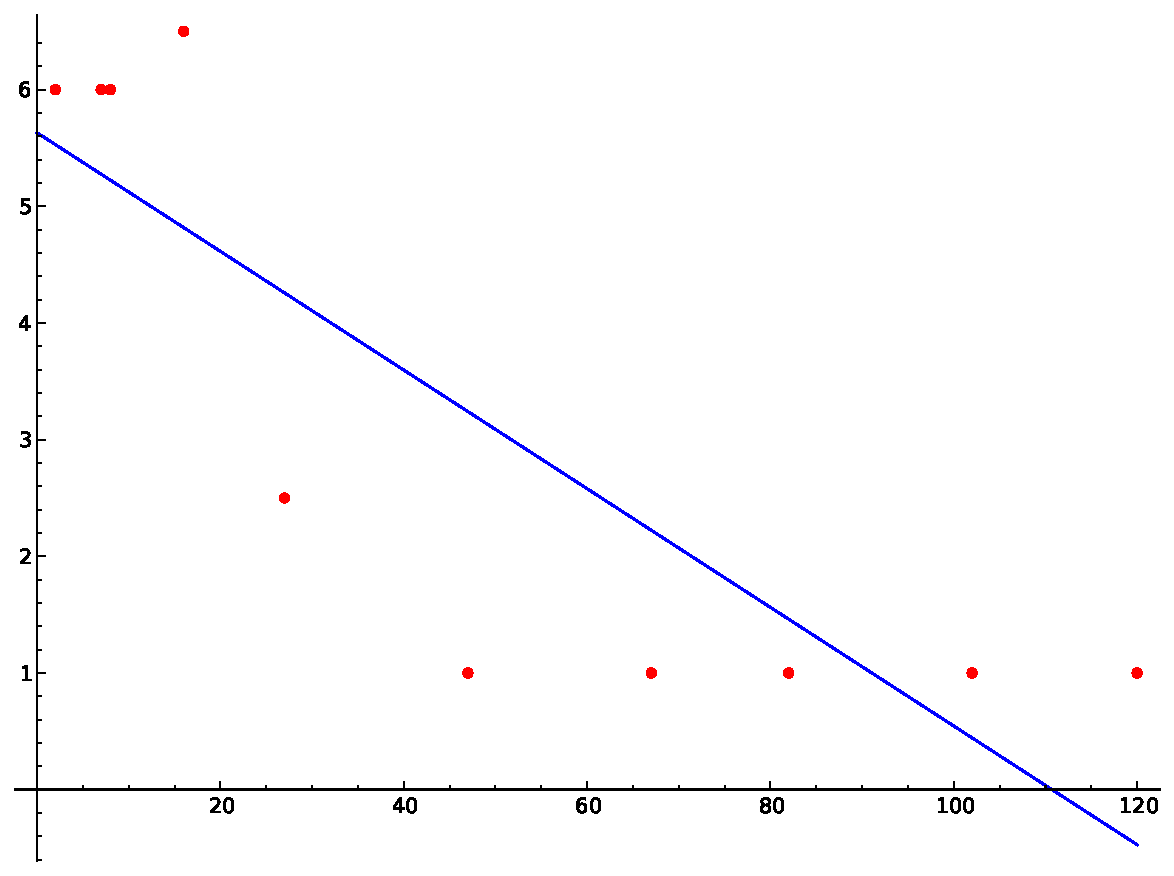
\includegraphics[width=.5\textwidth]{map/pix/bridges.pdf}
      \end{center}
      Tampaknya, model yang lebih baik adalah bahwa (dengan hanya satu
      pengecualian di antaranya) penyeberangan di dalam kota memiliki tarif yang
      kira-kira sama satu sama lain, demikian pula penyeberangan di utara negara
      bagian.
    \end{answer}
  \item 
    Ketika pesawat ulang-alik Challenger hancur pada 1986, salah satu kritik
    terhadap proses keputusan peluncuran NASA--Morton Thiokol adalah cara data
    gangguan atau kerusakan cincin-O dianalisis terhadap suhu.
    Tabel ini menghitung kejadian gangguan atau kerusakan, bukan empat kegagalan
    segel secara harfiah; kebocoran fatal terjadi pada sambungan belakang
    pendorong roket padat kanan yang gagal tersegel.
    Karena itu, ambang $y=4$ di bawah hanyalah ekstrapolasi matematis untuk
    latihan, bukan ambang keselamatan rekayasa.
    Tersedia data dari $24$ penerbangan sebelumnya.
    \begin{center}
      \begin{tabular}{r|rrrrrrrrrrr}
         \textit{suhu\ ${}^\circ$F}
            &53 &75 &57 &58 &63 &70 &70 &66 &67 &67 &67 \\
         \hline
         \textit{kegagalan}
            &3  &2  &1  &1  &1  &1  &1  &0  &0  &0  &0
      \end{tabular}\hspace*{3em}                                           \\
      \hspace*{3em}\begin{tabular}{|rrrrrrrrrrrrr}
                68 &69 &70 &70 &72 &73 &75 &76 &76 &78 &79 &80 &81\\
         \hline
                0  &0  &0  &0  &0  &0  &0  &0  &0  &0  &0  &0  &0
      \end{tabular}
    \end{center}
    Suhu pada hari itu diprakirakan \( 31^\circ\text{F} \).
    \begin{exparts}
      \partsitem Keputusan NASA untuk meluncurkan sebagian didasarkan pada grafik
        yang hanya menampilkan penerbangan dengan sekurang-kurangnya satu
        kegagalan cincin-O. Temukan garis yang paling cocok dengan ketujuh
        penerbangan tersebut. Berdasarkan data ini, prediksi banyak kegagalan
        cincin-O ketika suhu $31$, dan tentukan kapan banyak kegagalan akan
        melebihi empat.
      \partsitem Temukan garis yang paling cocok dengan seluruh $24$ penerbangan.
        Berdasarkan data tambahan ini, prediksi banyak kegagalan cincin-O ketika
        suhu $31$, dan tentukan kapan banyak kegagalan akan melebihi empat.
    \end{exparts}
    Menurut Anda, metode prediksi manakah yang lebih akurat?
    (Pembahasan yang sangat baik terdapat dalam \cite{Stats}.)
    \begin{answer}
      \begin{exparts}
        \partsitem Sistem aljabar komputer seperti Maple atau MuPAD memberikan
          intersep $b=4259/1398\approx 3.046495$ dan kemiringan
          $m=-71/2796\approx -0.025393419$.
          Substitusi $x=31$ ke dalam persamaan menghasilkan prediksi
          $y\approx 2.259299$, atau $2.26$ kejadian (dibulatkan ke dua tempat
          desimal).
          Substitusi $y=4$ dan penyelesaian persamaan memberikan suhu
          $x\approx -37.5493^\circ$F. Karena kemiringannya negatif, model
          memprediksi $y>4$ ketika $x<-37.55^\circ$F.
        \partsitem Berdasarkan informasi berikut,
          \begin{equation*}
            A =  
            \begin{mat}
               1 & 53 \\
               1 & 75 \\
%              1 & 57 \\
%              1 & 58 \\
%              1 & 63 \\
%              1 & 70 \\
%              1 & 70 \\
%              1 & 66 \\
%              1 & 67 \\
%              1 & 67 \\
%              1 & 67 \\
%              1 & 68 \\
%              1 & 69 \\
%              1 & 70 \\
%              1 & 70 \\
%              1 & 72 \\
%              1 & 73 \\
%              1 & 75 \\
%              1 & 76 \\
%              1 & 76 \\
%              1 & 78 \\
%              1 & 79 \\
               \vdots \\
               1 & 80 \\
               1 & 81
            \end{mat}
            \qquad
            \vec{b} =
            \colvec{ 3 \\
                     2 \\
%                    1 \\
%                    1 \\
%                    1 \\
%                    1 \\
%                    1 \\
%                    0 \\ 
%                    0 \\
%                    0 \\
%                    0 \\
%                    0 \\
%                    0 \\
%                    0 \\
%                    0 \\
%                    0 \\
%                    0 \\
%                    0 \\
%                    0 \\
%                    0 \\
%                    0 \\
%                    0 \\
                     \vdots \\
                     0 \\
                     0}
          \end{equation*}
          Maple memberikan intersep $b=187/40=4.675$ dan kemiringan
          $m=-73/1200\approx -0.060833$.
          Di sini, substitusi $x=31$ ke dalam persamaan memprediksi
          $y\approx 2.78917$, atau $2.79$ kejadian (dibulatkan ke dua tempat
          desimal).
          Substitusi $y=4$ memberikan suhu $x\approx 11.0959^\circ$F, dan model
          memprediksi $y>4$ pada suhu yang lebih rendah.
     \begin{center}  \small
       \includegraphics{map/mp/ch3.90}
      \end{center}
      \end{exparts}
      Model yang menggunakan seluruh $24$ penerbangan lebih layak karena
      membuang semua penerbangan tanpa gangguan berarti memilih data berdasarkan
      hasil dan menimbulkan bias. Meskipun demikian, kedua regresi linear ini
      tetap merupakan model risiko yang buruk: jumlah kejadian yang diprediksi
      tidak dibatasi dan data yang tersedia sedikit. Ambang hasil ekstrapolasi
      tidak boleh ditafsirkan sebagai suhu peluncuran yang aman.
    \end{answer}
  \item 
     Tabel berikut mencantumkan jarak rata-rata dari Matahari ke masing-masing
     tujuh planet pertama, dengan jarak rata-rata Bumi sebagai satuan.
     \begin{center}
       \begin{tabular}{ccccccc}
         Merkurius &Venus   &Bumi   &Mars    &Jupiter &Saturnus  &Uranus  \\
         \hline     
         $0.39$  &$0.72$  &$1.00$  &$1.52$  &$5.20$  &$9.54$  &$19.2$
       \end{tabular}
     \end{center}
    \begin{exparts}
      \partsitem Plot nomor planet (Merkurius adalah \( 1 \), dan seterusnya)
        terhadap jaraknya. Perhatikan bahwa plot tersebut tidak tampak seperti
        garis, sehingga mencari garis kecocokan terbaik tidak banyak berguna.
      \partsitem Namun, plot tersebut tampak seperti kurva eksponensial.
        Karena itu, plot nomor planet terhadap logaritma jaraknya.
        Apakah plot ini tampak seperti garis?
      \partsitem Dalam pola empiris ini, sabuk asteroid antara Mars dan Jupiter
        diperlakukan sebagai posisi ``planet yang hilang''.
        Nomori ulang sehingga Jupiter menjadi $6$, Saturnus menjadi $7$, dan
        Uranus menjadi $8$, lalu plot kembali terhadap logaritma.
        Apakah hasilnya tampak lebih baik?
      \partsitem Gunakan kuadrat terkecil pada data tersebut untuk memprediksi
        letak Neptunus.
      \partsitem Ulangi untuk memprediksi letak Pluto.
      \partsitem Apakah rumus tersebut akurat bagi Neptunus dan Pluto?
    \end{exparts}
    Pola empiris ini turut mendorong pencarian ``planet yang hilang'' di
    posisi~$5$ dan penemuan Ceres. Neptunus ditemukan melalui analisis gangguan
    orbit Uranus, bukan melalui metode ini. Lihat \cite{Gardner70}.
      \begin{answer}
        \begin{exparts}
          \partsitem Plotnya nonlinear.
            \begin{center}  \small
              \includegraphics{map/mp/ch3.91}
            \end{center}
          \partsitem Berikut plotnya.
           \begin{center}  \small
             \includegraphics{map/mp/ch3.92}
           \end{center}
            Mungkin terdapat lonjakan antara planet~$4$ dan planet~$5$.
          \partsitem Plot ini tampak lebih linear.
           \begin{center}  \small
             \includegraphics{map/mp/ch3.93}
           \end{center}
          \partsitem
            Dengan masukan berikut,
            \begin{equation*}
              A =  
              \begin{mat}[r]
                1 & 1 \\
                1 & 2 \\
                1 & 3 \\
                1 & 4 \\
                1 & 6 \\
                1 & 7 \\
                1 & 8
              \end{mat}
              \qquad
              \vec{b} = \colvec[r]{-0.40893539 \\
                          -0.1426675 \\
                           0 \\
                           0.18184359 \\
                           0.71600334 \\
                           0.97954837 \\
                           1.2833012}
            \end{equation*}
            MuPAD memberikan intersep $b= -0.6780677466$ dan kemiringan
            $m=0.2372763818$.
            Substitusi $x=9$ ke dalam persamaan
            $y= -0.6780677466+0.2372763818x$ memberikan logaritma jarak
            $1.4574197$, sehingga jarak Neptunus yang diperkirakan adalah
            $28.669472$.
          \partsitem Substitusi $x=10$ ke dalam persamaan yang sama memberikan
            logaritma jarak $1.6946961$, sehingga jarak Pluto yang diperkirakan
            adalah $49.510362$.
          \partsitem Jarak sebenarnya kira-kira $30.003$ bagi Neptunus dan
            $39.503$ bagi Pluto. Jadi, galat relatif prediksi masing-masing
            kira-kira $-4.44\%$ dan $+25.33\%$. Rumus tersebut cukup dekat bagi
            Neptunus, tetapi tidak akurat bagi Pluto.
        \end{exparts}
      \end{answer}
  % \item 
  %   William Bennett has proposed an Index of Leading Cultural Indicators
  %   for the US (\cite{Bennett}, in 1993).
  %   Among the statistics cited are the average daily hours spent watching TV, 
  %   and the average combined SAT scores.
  %   \begin{center}
  %     \begin{tabular}{r|cccccccc}
  %        &1960   &1965   &1970   &1975   &1980   &1985   &1990   &1992  
  %           \\ \hline
  %        \textit{TV}
  %        &5:06   &5:29   &5:56   &6:07   &6:36   &7:07   &6:55   &7:04 \\
  %        \textit{SAT}
  %        &$975$  &$969$  &$948$  &$910$  &$890$  &$906$  &$900$  &$899$ 
  %     \end{tabular} 
  %   \end{center}
  %   Suppose that a cause and effect relationship is proposed between
  %   the time spent watching TV and the decline in SAT scores (in this article,
  %   Mr.~Bennett does not argue that there is a direct connection).
  %   \begin{exparts}
  %    \partsitem Find the line of best fit relating the independent variable
  %      of average daily TV hours to the dependent variable of SAT scores.
  %    \partsitem Find the most recent estimate of the average daily TV hours  
  %      (Bennett's cites Neilsen Media Research as the source of these 
  %      estimates).
  %      Estimate the associated SAT score.
  %      How close is your estimate to the actual average?
  %      (Warning: a change has been made recently in the SAT,
  %      so you should investigate whether some adjustment needs to be made to
  %      the reported average to make a valid comparison.)
  %   \end{exparts}
  %   \begin{answer}
  %     \begin{exparts}
  %       \partsitem With this input
  %         \begin{equation*}
  %           A = 
  %           \begin{mat}[r]
  %             1 & 306 \\
  %             1 & 329 \\
  %             1 & 356 \\
  %             1 & 367 \\
  %             1 & 396 \\
  %             1 & 427 \\
  %             1 & 415 \\
  %             1 & 424
  %           \end{mat}
  %           \qquad
  %           b = 
  %           \colvec[r]{975 \\
  %                   969 \\
  %                   948 \\
  %                   910 \\
  %                   890 \\
  %                   906 \\
  %                   900 \\
  %                   899}
  %         \end{equation*}
  %         MAPLE gives the intercept 
  %         $b=34009779/28796\approx 1181.0591$ and the slope 
  %         $m=-19561/28796\approx -0.6793$.
  %         \begin{center}  \small
  %           \includegraphics{map/mp/ch3.94}
  %      \end{center}
  %     \end{exparts}
  %   \end{answer}
%  \item
%    Derive the 
%    \definend{normal equations}\index{least squares!normal equations}%
%    \index{normal equations!for least squares} for least squares line fitting:
%    for data points \( (x_1,y_1) \), \ldots, \( (x_n,y_n) \)
%    the line of best fit \( y=mx+b \) has this slope
%    \begin{equation*}
%      m=\frac{\frac{\displaystyle x_1y_1+\dots+x_ny_n}{\displaystyle n}
%              -(\frac{\displaystyle x_1+\dots+x_n}{\displaystyle n})
%               (\frac{\displaystyle y_1+\dots+y_n}{\displaystyle n})}{
%              \frac{\displaystyle {x_1}^2+\cdots+{x_n}^2}{\displaystyle n}
%              -(\frac{\displaystyle x_1+\dots+x_n}{\displaystyle n})^2}
%    \end{equation*}
%    and this vertical intercept.
%    \begin{equation*}
%      b=\frac{y_1+\dots+y_n}{n}-m(\frac{x_1+\dots+x_n}{n})
%    \end{equation*}
%    (\textit{Remark}.
%     A advantage of these equations is that a
%     person doing by-hand calculations can make up \Dash  and check \Dash  a 
%     table with a
%     column of $x_i$'s, one of $y_i$'s, one of $x_i^2$'s,
%     one of $y_i^2$'s , and finally one of $x_i\cdot y_i$'s.
%     Then the sums of these columns fit into the formulas.)
%     \begin{answer}
%       The $\nbyn{2}$ shows how the larger cases hold.
%     \end{answer}
\item Misalkan $W$ merupakan subruang dari $\Re^n$ bagi suatu~$n$, dan misalkan
  $\vec{v}$ bukan anggota~$W$.
  Misalkan proyeksi ortogonal $\vec{v}$ ke $W$ adalah vektor
  $\proj{\vec{v}}{W}=\vec{p}$.
  Tunjukkan bahwa $\vec{p}$ merupakan anggota~$W$ yang paling dekat dengan
  $\vec{v}$.
  \begin{answer}
    Bagi sebarang $\vec{w}\in W$, vektor $\vec{v}-\vec{p}$ dan
    $\vec{p}-\vec{w}$ saling ortogonal.
    Jadi, Teorema Pythagoras berlaku pada segitiga dengan kedua vektor tersebut
    sebagai kaki dan $\vec{v}-\vec{w}$ sebagai hipotenusa.
    Karena itu, $\vec{v}-\vec{w}$ sekurang-kurangnya sama panjang dengan
    $\vec{v}-\vec{p}$.
  \end{answer}

   





\end{exercises}
%\par\noindent\announcecomputercode %
%\begin{computercode}
%    #!/usr/bin/python
%    # least_squares.py   calculate the line of best fit for a data set
%    # data file format: each line is two numbers, x and y
%    import math, string
%
%    n = 0
%    sum__x = 0
%    sum_y = 0
%    sum_x_squared = 0
%    sum_xy = 0
%
%    fn = raw_input("Name of the data file? ")
%    datafile = open(fn,"r")
%    while 1:
%      ln = datafile.readline()
%      if (ln):
%            data = string.split(ln)
%            x = string.atof(data[0])
%            y = string.atof(data[1])
%            n = n+1
%            sum_x = sum_x+x
%            sum_y = sum_y+y
%            sum_x_squared = sum_x_squared+(x*x)
%            sum_xy = sum_xy +(x*y)
%      else:
%            break
%    datafile.close()
%
%    slope=(sum_of_xy-pow(sum_x,2)/n)/(sum_x_squared-pow(sum_x,2)/n)
%    intercept=(sum_y-(slope*sum_x))/n
%    print "line of best fit: slope=",slope," intercept=",intercept 
%\end{computercode}


\index{garis kecocokan terbaik|)}
\index{kuadrat terkecil|)}
